\chapter*{LAMPIRAN}

\section{Block Design Sistem OV7670, DDR3, dan VGA}

    \begin{figure}[H]
        \centering
        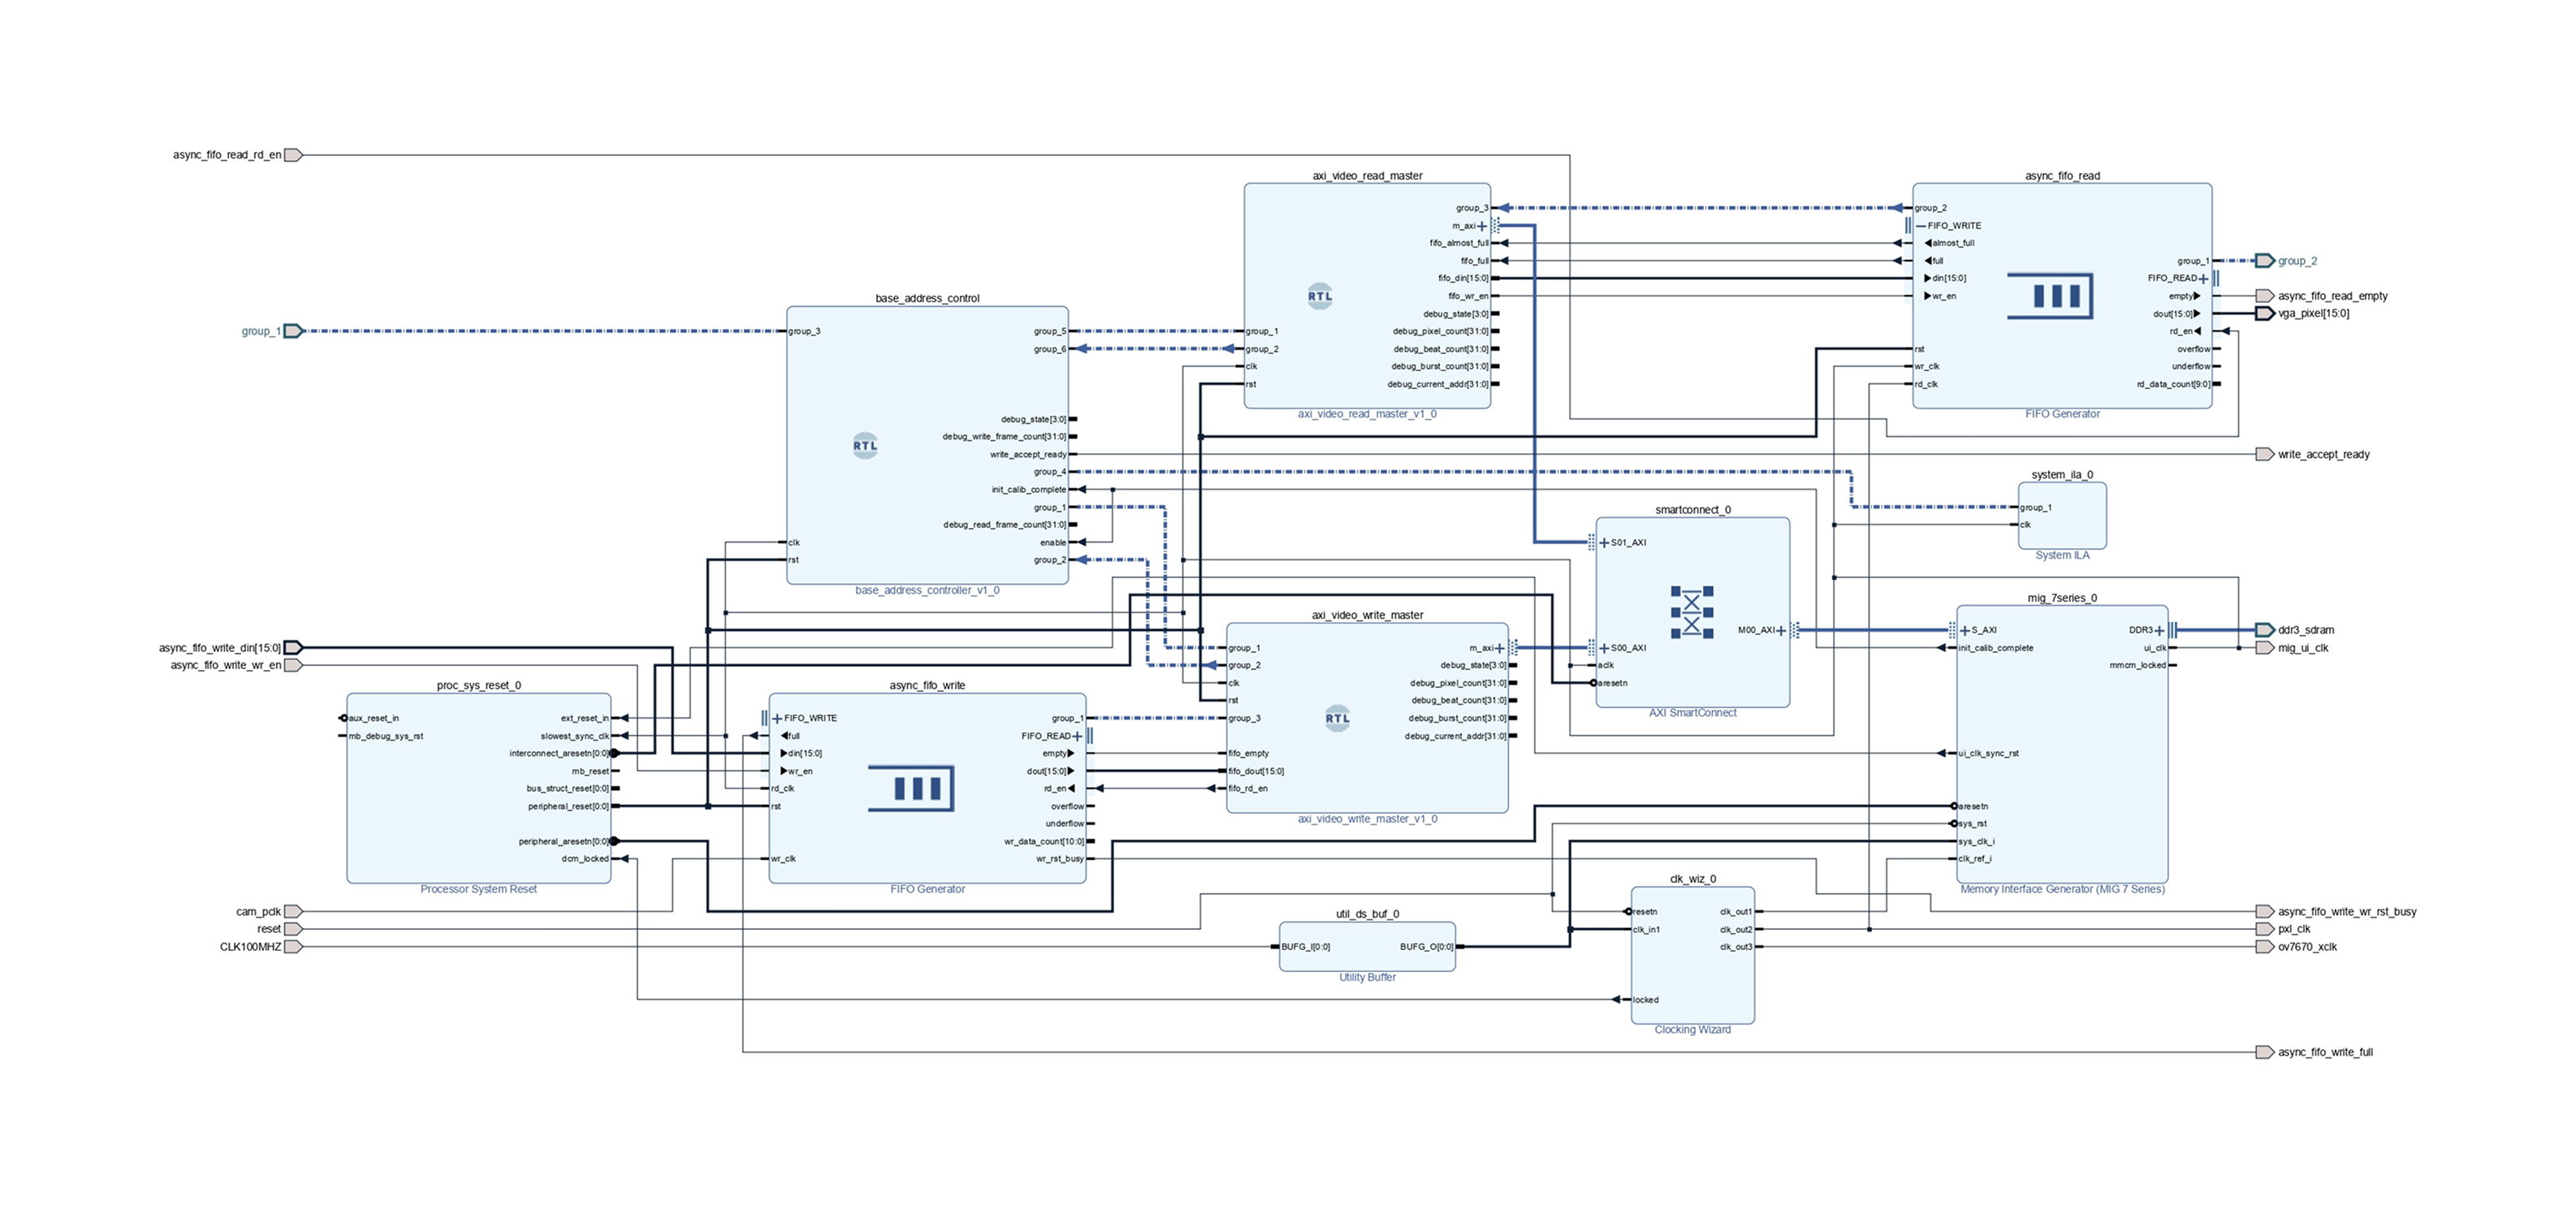
\includegraphics[width=0.95\textwidth]{gambar/block-design-camera-ddr-vga.png}
        \caption{Block Design Alur Inferensi Camera Sampai VGA}
        \label{fig:bd-cam-ddr-vga}
    \end{figure}

\section{Kode Implementasi Kuantitasi Parameter 16 Bit}
	\begin{lstlisting}[language=Python, title={Kode Kuantisasi 16 bit parameter model}, label={code:quantitize model parameter}]

def quantize_signed(x, bits, frac_bits):
    q = np.round(x * (1 << frac_bits)).astype(np.int64)
    min_q = -(1 << (bits - 1))
    max_q =  (1 << (bits - 1)) - 1
    sat_low = int(np.sum(q < min_q))
    sat_high = int(np.sum(q > max_q))
    q = np.clip(q, min_q, max_q)
    return q.astype(np.int64), sat_low, sat_high

def to_twos_hex(v, bits):
    v = int(v)
    if v < 0:
        v = (1 << bits) + v
    return f"{v:0{bits//4}X}"

def save_mem(path, q, bits):
    flat = q.reshape(-1)
    with open(path, "w") as f:
        for v in flat:
            f.write(to_twos_hex(v, bits) + "\n")
    print(f"saved: {path} lines={len(flat)} bits={bits}")

def report(name, arr, q, lo, hi):
    print(f"\n{name}")
    print("  shape:", arr.shape)
    print("  float min/max:", float(np.min(arr)), float(np.max(arr)))
    print("  quant min/max:", int(np.min(q)), int(np.max(q)))
    print("  saturation low/high:", lo, hi)

	\end{lstlisting}

\section{Kode Evaluasi Hasil Perbedaan Bit}

	\begin{lstlisting}[language=Python, title={Kode evaluasi perbedaan bit Python dan Verilog}, label={code:bit-difference-eval}]

import numpy as np
import pandas as pd

def sign_extend(arr, bit_width):
    """
    Untuk mengubah unsigned two's complement menjadi signed integer.
    Contoh kalau ACT_SIZE = 24, maka bit_width = 24.
    """
    arr = arr.astype(np.int64)

    if bit_width is None:
        return arr

    sign_bit = 1 << (bit_width - 1)
    full_range = 1 << bit_width

    return np.where(arr >= sign_bit, arr - full_range, arr)


def python_float_to_fixed(arr, frac_bits=14, mode="round"):
    """
    Convert float Python ke fixed-point integer.
    """
    scale = 1 << frac_bits
    scaled = arr * scale

    if mode == "round":
        return np.round(scaled).astype(np.int64)

    elif mode == "trunc":
        return np.trunc(scaled).astype(np.int64)

    elif mode == "floor":
        return np.floor(scaled).astype(np.int64)

    else:
        raise ValueError("mode harus 'round', 'trunc', atau 'floor'")


def compare_numpy_vs_verilog(
    python_res,
    verilog_res,
    row_count,
    channel_count,
    prefix="ch",
    frac_bits=14,
    bit_width=24,
    verilog_is_fixed=True,
    quant_mode="round"
):
    """
    Membandingkan hasil NumPy Python vs hasil Verilog/Icarus.

    python_res:
        shape (row_count, channel_count)
        biasanya float

    verilog_res:
        shape (row_count, channel_count)
        biasanya integer fixed-point dari Verilog

    Output dataframe:
        ch0_verilog, ch0_python, ..., ch7_verilog, ch7_python, float_diff, bit_diff
    """

    python_res = np.asarray(python_res, dtype=np.float64)
    verilog_res = np.asarray(verilog_res)

    expected_shape = (row_count, channel_count)

    if python_res.shape != expected_shape:
        raise ValueError(
            f"Shape python_res salah. Dapat {python_res.shape}, expected {expected_shape}"
        )

    if verilog_res.shape != expected_shape:
        raise ValueError(
            f"Shape verilog_res salah. Dapat {verilog_res.shape}, expected {expected_shape}"
        )

    if verilog_is_fixed:
        verilog_fixed = verilog_res.astype(np.int64)

        # gunakan ini kalau output Verilog adalah raw two's complement
        verilog_fixed = sign_extend(verilog_fixed, bit_width)

        verilog_float = verilog_fixed.astype(np.float64) / (1 << frac_bits)

    else:
        # kalau Verilog sudah menulis float
        verilog_float = verilog_res.astype(np.float64)
        verilog_fixed = python_float_to_fixed(
            verilog_float,
            frac_bits=frac_bits,
            mode=quant_mode
        )

    python_fixed = python_float_to_fixed(
        python_res,
        frac_bits=frac_bits,
        mode=quant_mode
    )

    float_diff_per_ch = np.abs(python_res - verilog_float)
    bit_diff_per_ch = np.abs(python_fixed - verilog_fixed)

    # Satu row punya banyak channel.
    # Maka float_diff dan bit_diff di sini adalah diff maksimum dari semua channel pada row itu.
    float_diff = np.max(float_diff_per_ch, axis=1)
    bit_diff = np.max(bit_diff_per_ch, axis=1)

    data = {}

    for ch in range(channel_count):
        data[f"{prefix}{ch}_verilog"] = verilog_float[:, ch]
        data[f"{prefix}{ch}_python"] = python_res[:, ch]

    data["float_diff"] = float_diff
    data["bit_diff"] = bit_diff

    df = pd.DataFrame(data)

    return df
	\end{lstlisting}

\section{Kode Verilog \emph{AXI Read}}

    \begin{lstlisting}[language=Verilog, title={Kode \emph{AXI Read} Yang akan mengisi \emph{FIFO VGA}}, label={code:verilog-axi-read}]

`timescale 1ns / 1ps

module axi_video_read_master #(
    parameter AXI_ADDR_WIDTH   = 32,
    parameter AXI_DATA_WIDTH   = 64,
    parameter AXI_ID_WIDTH     = 4,

    parameter PIXEL_BITS       = 16,

    parameter FRAME_WIDTH      = 640,
    parameter FRAME_HEIGHT     = 480,

    // Untuk MIG AXI 64-bit, aman pakai burst 8.
    parameter BURST_LEN        = 8,

    // Sesuai FIFO Generator kamu:
    // wr_data_count width = 10-bit
    parameter FIFO_COUNT_WIDTH = 10,

    // FIFO depth efektif untuk count 10-bit.
    // Walaupun di GUI kamu tulis 1028, count 10-bit praktis dipakai sebagai 1024 level.
    parameter FIFO_DEPTH_WORDS = 1024,

    // Margin supaya tidak terlalu dekat full.
    parameter FIFO_SAFE_MARGIN = 8,

    parameter AXI_ID_VALUE     = 0
)(
    input  wire                         clk,
    input  wire                         rst,          // active-high, sync to clk

    input  wire                         enable,
    input  wire                         frame_start,  // pulse 1 clock
    input  wire [AXI_ADDR_WIDTH-1:0]    frame_base_addr,

    output reg  [PIXEL_BITS-1:0]        fifo_din,
    output reg                          fifo_wr_en,
    input  wire                         fifo_full,
    input  wire                         fifo_almost_full,
    input  wire [FIFO_COUNT_WIDTH-1:0]  fifo_wr_data_count,
    input  wire                         fifo_wr_rst_busy,

    // ============================================================
    // AXI4 Read Address Channel
    // ============================================================
    output wire [AXI_ID_WIDTH-1:0]      m_axi_arid,
    output reg  [AXI_ADDR_WIDTH-1:0]    m_axi_araddr,
    output wire [7:0]                   m_axi_arlen,
    output wire [2:0]                   m_axi_arsize,
    output wire [1:0]                   m_axi_arburst,
    output wire                         m_axi_arlock,
    output wire [3:0]                   m_axi_arcache,
    output wire [2:0]                   m_axi_arprot,
    output wire [3:0]                   m_axi_arqos,
    output reg                          m_axi_arvalid,
    input  wire                         m_axi_arready,

    // ============================================================
    // AXI4 Read Data Channel
    // ============================================================
    input  wire [AXI_ID_WIDTH-1:0]      m_axi_rid,
    input  wire [AXI_DATA_WIDTH-1:0]    m_axi_rdata,
    input  wire [1:0]                   m_axi_rresp,
    input  wire                         m_axi_rlast,
    input  wire                         m_axi_rvalid,
    output reg                          m_axi_rready,

    // ============================================================
    // Status / debug
    // ============================================================
    output reg                          busy,
    output reg                          done,
    output reg                          error,
    output reg  [3:0]                   debug_state,
    output reg  [31:0]                  debug_pixel_count,
    output reg  [31:0]                  debug_beat_count,
    output reg  [31:0]                  debug_burst_count,
    output reg  [AXI_ADDR_WIDTH-1:0]    debug_current_addr
);

    // ============================================================
    // Local parameters
    // ============================================================
    localparam integer BYTES_PER_BEAT    = AXI_DATA_WIDTH / 8;
    localparam integer PIXELS_PER_BEAT   = AXI_DATA_WIDTH / PIXEL_BITS;
    localparam integer FRAME_PIXELS      = FRAME_WIDTH * FRAME_HEIGHT;
    localparam integer FRAME_BEATS       = FRAME_PIXELS / PIXELS_PER_BEAT;
    localparam integer PIXELS_PER_BURST  = BURST_LEN * PIXELS_PER_BEAT;
    localparam integer ADDR_STEP_BURST   = BURST_LEN * BYTES_PER_BEAT;

    localparam integer FIFO_START_LEVEL  =
        FIFO_DEPTH_WORDS - PIXELS_PER_BURST - FIFO_SAFE_MARGIN;

    // Untuk konfigurasi sekarang:
    // AXI_DATA_WIDTH   = 64
    // BYTES_PER_BEAT   = 8
    // PIXELS_PER_BEAT  = 4
    // BURST_LEN        = 8
    // PIXELS_PER_BURST = 32
    // ADDR_STEP_BURST  = 64 byte

    // ============================================================
    // AXI size encoder
    // AXI ARSIZE:
    // 000 = 1 byte
    // 001 = 2 byte
    // 010 = 4 byte
    // 011 = 8 byte  -> 64-bit
    // 100 = 16 byte -> 128-bit
    // ============================================================
    function [2:0] axi_size_from_bytes;
        input integer bytes;
        begin
            case (bytes)
                1:   axi_size_from_bytes = 3'b000;
                2:   axi_size_from_bytes = 3'b001;
                4:   axi_size_from_bytes = 3'b010;
                8:   axi_size_from_bytes = 3'b011;
                16:  axi_size_from_bytes = 3'b100;
                32:  axi_size_from_bytes = 3'b101;
                64:  axi_size_from_bytes = 3'b110;
                128: axi_size_from_bytes = 3'b111;
                default: axi_size_from_bytes = 3'b000;
            endcase
        end
    endfunction

    // ============================================================
    // State encoding
    // ============================================================
    localparam [3:0]
        S_IDLE        = 4'd0,
        S_WAIT_SPACE  = 4'd1,
        S_AR          = 4'd2,
        S_R           = 4'd3,
        S_UNPACK      = 4'd4,
        S_DONE        = 4'd5,
        S_ERROR       = 4'd6;

    reg [3:0] state;

    reg [AXI_ADDR_WIDTH-1:0] addr_reg;

    reg [31:0] pixel_count;
    reg [31:0] beat_count_total;
    reg [31:0] burst_count_total;

    reg [7:0]  beat_index_in_burst;
    reg [3:0]  unpack_index;

    reg [AXI_DATA_WIDTH-1:0] read_data_reg;
    reg                      read_last_reg;

    wire [31:0] fifo_used_words;
    wire        fifo_has_space_for_burst;

    assign fifo_used_words = fifo_wr_data_count;

    assign fifo_has_space_for_burst =
        (!fifo_full) &&
        (!fifo_almost_full) &&
        (!fifo_wr_rst_busy) &&
        (fifo_used_words <= FIFO_START_LEVEL);

    // ============================================================
    // AXI constant signals
    // ============================================================
    assign m_axi_arid    = AXI_ID_VALUE;
    assign m_axi_arlen   = BURST_LEN - 1;
    assign m_axi_arsize  = axi_size_from_bytes(BYTES_PER_BEAT);
    assign m_axi_arburst = 2'b01;        // INCR burst
    assign m_axi_arlock  = 1'b0;
    assign m_axi_arcache = 4'b0011;
    assign m_axi_arprot  = 3'b000;
    assign m_axi_arqos   = 4'b0000;

    // ============================================================
    // Main FSM
    // ============================================================
    always @(posedge clk) begin
        if (rst) begin
            state                <= S_IDLE;

            fifo_din             <= {PIXEL_BITS{1'b0}};
            fifo_wr_en           <= 1'b0;

            m_axi_araddr         <= {AXI_ADDR_WIDTH{1'b0}};
            m_axi_arvalid        <= 1'b0;
            m_axi_rready         <= 1'b0;

            busy                 <= 1'b0;
            done                 <= 1'b0;
            error                <= 1'b0;
            debug_state          <= S_IDLE;

            addr_reg             <= {AXI_ADDR_WIDTH{1'b0}};

            pixel_count          <= 32'd0;
            beat_count_total     <= 32'd0;
            burst_count_total    <= 32'd0;

            beat_index_in_burst  <= 8'd0;
            unpack_index         <= 4'd0;

            read_data_reg        <= {AXI_DATA_WIDTH{1'b0}};
            read_last_reg        <= 1'b0;

            debug_pixel_count    <= 32'd0;
            debug_beat_count     <= 32'd0;
            debug_burst_count    <= 32'd0;
            debug_current_addr   <= {AXI_ADDR_WIDTH{1'b0}};
        end else begin
            // Default pulse
            fifo_wr_en  <= 1'b0;
            done        <= 1'b0;
            debug_state <= state;

            case (state)

                // IDLE
                // Menunggu frame_start dari base_address_controller.
                S_IDLE: begin
                    busy          <= 1'b0;
                    error         <= 1'b0;

                    m_axi_arvalid <= 1'b0;
                    m_axi_rready  <= 1'b0;

                    fifo_wr_en    <= 1'b0;

                    if (enable && frame_start && !fifo_wr_rst_busy) begin
                        busy                 <= 1'b1;

                        addr_reg             <= frame_base_addr;
                        m_axi_araddr         <= frame_base_addr;
                        debug_current_addr   <= frame_base_addr;

                        pixel_count          <= 32'd0;
                        beat_count_total     <= 32'd0;
                        burst_count_total    <= 32'd0;

                        beat_index_in_burst  <= 8'd0;
                        unpack_index         <= 4'd0;

                        read_data_reg        <= {AXI_DATA_WIDTH{1'b0}};
                        read_last_reg        <= 1'b0;

                        debug_pixel_count    <= 32'd0;
                        debug_beat_count     <= 32'd0;
                        debug_burst_count    <= 32'd0;

                        state                <= S_WAIT_SPACE;
                    end
                end

                S_WAIT_SPACE: begin
                    m_axi_rready <= 1'b0;

                    if (!enable) begin
                        state <= S_IDLE;
                    end else if (beat_count_total >= FRAME_BEATS) begin
                        state <= S_DONE;
                    end else if (fifo_has_space_for_burst) begin
                        m_axi_araddr   <= addr_reg;
                        m_axi_arvalid  <= 1'b1;
                        debug_current_addr <= addr_reg;
                        state          <= S_AR;
                    end
                end

                S_AR: begin
                    if (m_axi_arvalid && m_axi_arready) begin
                        m_axi_arvalid       <= 1'b0;

                        beat_index_in_burst <= 8'd0;
                        unpack_index        <= 4'd0;

                        // Siap menerima data read dari AXI.
                        m_axi_rready        <= 1'b1;

                        state               <= S_R;
                    end else if (!enable) begin
                        // Belum handshake, jadi aman batal.
                        m_axi_arvalid <= 1'b0;
                        m_axi_rready  <= 1'b0;
                        busy          <= 1'b0;
                        state         <= S_IDLE;
                    end
                end

                S_R: begin
                    if (m_axi_rvalid && m_axi_rready) begin
                        m_axi_rready  <= 1'b0;

                        read_data_reg <= m_axi_rdata;
                        read_last_reg <= m_axi_rlast;

                        if (m_axi_rresp != 2'b00) begin
                            error <= 1'b1;
                            state <= S_ERROR;
                        end else begin
                            unpack_index <= 4'd0;
                            state        <= S_UNPACK;
                        end
                    end
                end

                S_UNPACK: begin
                    if (!fifo_full && !fifo_wr_rst_busy) begin
                        fifo_din   <= read_data_reg[unpack_index*PIXEL_BITS +: PIXEL_BITS];
                        fifo_wr_en <= 1'b1;

                        pixel_count <= pixel_count + 32'd1;

                        if (unpack_index == PIXELS_PER_BEAT - 1) begin
                            unpack_index     <= 4'd0;
                            beat_count_total <= beat_count_total + 32'd1;

                            // Cek RLAST:
                            // RLAST harus muncul hanya pada beat terakhir burst.
                            if ((read_last_reg && (beat_index_in_burst != BURST_LEN - 1)) ||
                                (!read_last_reg && (beat_index_in_burst == BURST_LEN - 1))) begin
                                error <= 1'b1;
                                state <= S_ERROR;
                            end else begin
                                if (beat_index_in_burst == BURST_LEN - 1) begin
                                    // Satu burst selesai.
                                    burst_count_total <= burst_count_total + 32'd1;

                                    addr_reg <= addr_reg + ADDR_STEP_BURST;
                                    debug_current_addr <= addr_reg + ADDR_STEP_BURST;

                                    beat_index_in_burst <= 8'd0;
                                    m_axi_rready        <= 1'b0;

                                    if ((beat_count_total + 32'd1) >= FRAME_BEATS) begin
                                        state <= S_DONE;
                                    end else begin
                                        state <= S_WAIT_SPACE;
                                    end
                                end else begin
                                    // Masih ada beat berikutnya dalam burst ini.
                                    beat_index_in_burst <= beat_index_in_burst + 8'd1;

                                    // Siap menerima beat AXI berikutnya.
                                    m_axi_rready <= 1'b1;
                                    state        <= S_R;
                                end
                            end
                        end else begin
                            unpack_index <= unpack_index + 4'd1;
                        end
                    end
                end

                S_DONE: begin
                    busy <= 1'b0;
                    done <= 1'b1;

                    m_axi_arvalid <= 1'b0;
                    m_axi_rready  <= 1'b0;
                    fifo_wr_en    <= 1'b0;

                    debug_pixel_count <= pixel_count;
                    debug_beat_count  <= beat_count_total;
                    debug_burst_count <= burst_count_total;

                    state <= S_IDLE;
                end

                S_ERROR: begin
                    busy <= 1'b0;
                    done <= 1'b0;

                    m_axi_arvalid <= 1'b0;
                    m_axi_rready  <= 1'b0;
                    fifo_wr_en    <= 1'b0;

                    debug_pixel_count <= pixel_count;
                    debug_beat_count  <= beat_count_total;
                    debug_burst_count <= burst_count_total;

                    // Tetap di error sampai reset.
                    state <= S_ERROR;
                end

                default: begin
                    state <= S_IDLE;
                end

            endcase
        end
    end

endmodule

	\end{lstlisting}

\section{Kode Verilog \emph{AXI Write}}

    \begin{lstlisting}[language=Verilog, title={Kode \emph{AXI Write} Yang akan membaca \emph{FIFO Camera} dan menulis ke \emph{DDR3 SDRAM}}, label={code:verilog-axi-write}]

`timescale 1ns / 1ps

module axi_video_write_master #(
    parameter AXI_ADDR_WIDTH   = 32,
    parameter AXI_DATA_WIDTH   = 64,
    parameter AXI_ID_WIDTH     = 4,

    parameter PIXEL_BITS       = 16,

    parameter FRAME_WIDTH      = 640,
    parameter FRAME_HEIGHT     = 480,

    parameter BURST_LEN        = 8,

    // Sesuai FIFO Generator kamu:
    // rd_data_count width = 10-bit
    parameter FIFO_COUNT_WIDTH = 10,

    parameter AXI_ID_VALUE     = 0
)(
    input  wire                         clk,
    input  wire                         rst,          // active-high, sync to clk

    input  wire                         enable,
    input  wire                         frame_start,  // pulse 1 clock
    input  wire [AXI_ADDR_WIDTH-1:0]    frame_base_addr,

    input  wire [PIXEL_BITS-1:0]        fifo_dout,
    input  wire                         fifo_empty,
    input  wire                         fifo_valid,
    input  wire [FIFO_COUNT_WIDTH-1:0]  fifo_rd_data_count,
    input  wire                         fifo_rd_rst_busy,
    output reg                          fifo_rd_en,


    output wire [AXI_ID_WIDTH-1:0]      m_axi_awid,
    output reg  [AXI_ADDR_WIDTH-1:0]    m_axi_awaddr,
    output wire [7:0]                   m_axi_awlen,
    output wire [2:0]                   m_axi_awsize,
    output wire [1:0]                   m_axi_awburst,
    output wire                         m_axi_awlock,
    output wire [3:0]                   m_axi_awcache,
    output wire [2:0]                   m_axi_awprot,
    output wire [3:0]                   m_axi_awqos,
    output reg                          m_axi_awvalid,
    input  wire                         m_axi_awready,


    output reg  [AXI_DATA_WIDTH-1:0]    m_axi_wdata,
    output wire [AXI_DATA_WIDTH/8-1:0]  m_axi_wstrb,
    output reg                          m_axi_wlast,
    output reg                          m_axi_wvalid,
    input  wire                         m_axi_wready,

    // ============================================================
    // AXI4 Write Response Channel
    // ============================================================
    input  wire [AXI_ID_WIDTH-1:0]      m_axi_bid,
    input  wire [1:0]                   m_axi_bresp,
    input  wire                         m_axi_bvalid,
    output reg                          m_axi_bready,

    // ============================================================
    // Status / debug
    // ============================================================
    output reg                          busy,
    output reg                          done,
    output reg                          error,
    output reg  [3:0]                   debug_state,
    output reg  [31:0]                  debug_pixel_count,
    output reg  [31:0]                  debug_beat_count,
    output reg  [31:0]                  debug_burst_count,
    output reg  [AXI_ADDR_WIDTH-1:0]    debug_current_addr
);

    // ============================================================
    // Local parameters
    // ============================================================
    localparam integer BYTES_PER_BEAT    = AXI_DATA_WIDTH / 8;
    localparam integer PIXELS_PER_BEAT   = AXI_DATA_WIDTH / PIXEL_BITS;
    localparam integer FRAME_PIXELS      = FRAME_WIDTH * FRAME_HEIGHT;
    localparam integer FRAME_BEATS       = FRAME_PIXELS / PIXELS_PER_BEAT;
    localparam integer PIXELS_PER_BURST  = BURST_LEN * PIXELS_PER_BEAT;
    localparam integer ADDR_STEP_BURST   = BURST_LEN * BYTES_PER_BEAT;

    // Untuk konfigurasi sekarang:
    // AXI_DATA_WIDTH   = 64
    // BYTES_PER_BEAT   = 8
    // PIXELS_PER_BEAT  = 4
    // BURST_LEN        = 8
    // PIXELS_PER_BURST = 32
    // ADDR_STEP_BURST  = 64 byte


    function [2:0] axi_size_from_bytes;
        input integer bytes;
        begin
            case (bytes)
                1:   axi_size_from_bytes = 3'b000;
                2:   axi_size_from_bytes = 3'b001;
                4:   axi_size_from_bytes = 3'b010;
                8:   axi_size_from_bytes = 3'b011;
                16:  axi_size_from_bytes = 3'b100;
                32:  axi_size_from_bytes = 3'b101;
                64:  axi_size_from_bytes = 3'b110;
                128: axi_size_from_bytes = 3'b111;
                default: axi_size_from_bytes = 3'b000;
            endcase
        end
    endfunction

    // ============================================================
    // State encoding
    // ============================================================
    localparam [3:0]
        S_IDLE       = 4'd0,
        S_WAIT_FIFO  = 4'd1,
        S_AW         = 4'd2,
        S_PACK       = 4'd3,
        S_W          = 4'd4,
        S_B          = 4'd5,
        S_DONE       = 4'd6,
        S_ERROR      = 4'd7;

    reg [3:0] state;

    reg [AXI_ADDR_WIDTH-1:0] addr_reg;

    reg [31:0] pixel_count;
    reg [31:0] beat_count_total;
    reg [31:0] burst_count_total;

    reg [7:0]  beat_index_in_burst;
    reg [3:0]  pack_index;

    reg [AXI_DATA_WIDTH-1:0] pack_reg;

    // ============================================================
    // AXI constant signals
    // ============================================================
    assign m_axi_awid    = AXI_ID_VALUE;
    assign m_axi_awlen   = BURST_LEN - 1;
    assign m_axi_awsize  = axi_size_from_bytes(BYTES_PER_BEAT);
    assign m_axi_awburst = 2'b01;        // INCR burst
    assign m_axi_awlock  = 1'b0;
    assign m_axi_awcache = 4'b0011;
    assign m_axi_awprot  = 3'b000;
    assign m_axi_awqos   = 4'b0000;

    assign m_axi_wstrb   = {BYTES_PER_BEAT{1'b1}};

    // ============================================================
    // Main FSM
    // ============================================================
    always @(posedge clk) begin
        if (rst) begin
            state                 <= S_IDLE;

            fifo_rd_en            <= 1'b0;

            m_axi_awaddr          <= {AXI_ADDR_WIDTH{1'b0}};
            m_axi_awvalid         <= 1'b0;

            m_axi_wdata           <= {AXI_DATA_WIDTH{1'b0}};
            m_axi_wlast           <= 1'b0;
            m_axi_wvalid          <= 1'b0;

            m_axi_bready          <= 1'b0;

            busy                  <= 1'b0;
            done                  <= 1'b0;
            error                 <= 1'b0;
            debug_state           <= S_IDLE;

            addr_reg              <= {AXI_ADDR_WIDTH{1'b0}};

            pixel_count           <= 32'd0;
            beat_count_total      <= 32'd0;
            burst_count_total     <= 32'd0;

            beat_index_in_burst   <= 8'd0;
            pack_index            <= 4'd0;
            pack_reg              <= {AXI_DATA_WIDTH{1'b0}};

            debug_pixel_count     <= 32'd0;
            debug_beat_count      <= 32'd0;
            debug_burst_count     <= 32'd0;
            debug_current_addr    <= {AXI_ADDR_WIDTH{1'b0}};
        end else begin
            // Default pulse
            fifo_rd_en  <= 1'b0;
            done        <= 1'b0;
            debug_state <= state;

            case (state)

                S_IDLE: begin
                    busy          <= 1'b0;
                    error         <= 1'b0;

                    m_axi_awvalid <= 1'b0;
                    m_axi_wvalid  <= 1'b0;
                    m_axi_wlast   <= 1'b0;
                    m_axi_bready  <= 1'b0;

                    fifo_rd_en    <= 1'b0;

                    if (enable && frame_start && !fifo_rd_rst_busy) begin
                        busy                  <= 1'b1;

                        addr_reg              <= frame_base_addr;
                        m_axi_awaddr          <= frame_base_addr;
                        debug_current_addr    <= frame_base_addr;

                        pixel_count           <= 32'd0;
                        beat_count_total      <= 32'd0;
                        burst_count_total     <= 32'd0;

                        beat_index_in_burst   <= 8'd0;
                        pack_index            <= 4'd0;
                        pack_reg              <= {AXI_DATA_WIDTH{1'b0}};

                        debug_pixel_count     <= 32'd0;
                        debug_beat_count      <= 32'd0;
                        debug_burst_count     <= 32'd0;

                        state                 <= S_WAIT_FIFO;
                    end
                end

                S_WAIT_FIFO: begin
                    if (!enable) begin
                        state <= S_IDLE;
                    end else if (fifo_rd_rst_busy) begin
                        state <= S_WAIT_FIFO;
                    end else if (beat_count_total >= FRAME_BEATS) begin
                        state <= S_DONE;
                    end else if (fifo_rd_data_count >= PIXELS_PER_BURST) begin
                        m_axi_awaddr      <= addr_reg;
                        debug_current_addr <= addr_reg;
                        m_axi_awvalid     <= 1'b1;
                        state             <= S_AW;
                    end
                end

                S_AW: begin
                    if (m_axi_awvalid && m_axi_awready) begin
                        m_axi_awvalid       <= 1'b0;

                        beat_index_in_burst <= 8'd0;
                        pack_index          <= 4'd0;
                        pack_reg            <= {AXI_DATA_WIDTH{1'b0}};

                        state               <= S_PACK;
                    end
                end

                S_PACK: begin
                    if (!enable) begin
                        state <= S_IDLE;
                    end else if (fifo_valid && !fifo_empty && !fifo_rd_rst_busy) begin
                        fifo_rd_en <= 1'b1;

                        pack_reg[pack_index*PIXEL_BITS +: PIXEL_BITS] <= fifo_dout;
                        pixel_count <= pixel_count + 32'd1;

                        if (pack_index == PIXELS_PER_BEAT - 1) begin
                            // Kirim beat yang sudah lengkap.
                            // Karena assignment non-blocking, slice terakhir
                            // ditulis langsung juga ke m_axi_wdata.
                            m_axi_wdata <= pack_reg;
                            m_axi_wdata[pack_index*PIXEL_BITS +: PIXEL_BITS] <= fifo_dout;

                            m_axi_wvalid <= 1'b1;
                            m_axi_wlast  <= (beat_index_in_burst == BURST_LEN - 1);

                            pack_index   <= 4'd0;
                            state        <= S_W;
                        end else begin
                            pack_index <= pack_index + 4'd1;
                        end
                    end
                end

                S_W: begin
                    if (m_axi_wvalid && m_axi_wready) begin
                        m_axi_wvalid <= 1'b0;
                        m_axi_wlast  <= 1'b0;

                        beat_count_total <= beat_count_total + 32'd1;

                        if (beat_index_in_burst == BURST_LEN - 1) begin
                            beat_index_in_burst <= 8'd0;
                            m_axi_bready        <= 1'b1;
                            state               <= S_B;
                        end else begin
                            beat_index_in_burst <= beat_index_in_burst + 8'd1;
                            pack_reg            <= {AXI_DATA_WIDTH{1'b0}};
                            pack_index          <= 4'd0;
                            state               <= S_PACK;
                        end
                    end
                end

                S_B: begin
                    if (m_axi_bvalid && m_axi_bready) begin
                        m_axi_bready <= 1'b0;

                        if (m_axi_bresp != 2'b00) begin
                            error <= 1'b1;
                            state <= S_ERROR;
                        end else begin
                            burst_count_total <= burst_count_total + 32'd1;
                            addr_reg          <= addr_reg + ADDR_STEP_BURST;
                            debug_current_addr <= addr_reg + ADDR_STEP_BURST;

                            if (beat_count_total >= FRAME_BEATS) begin
                                state <= S_DONE;
                            end else begin
                                state <= S_WAIT_FIFO;
                            end
                        end
                    end
                end

                S_DONE: begin
                    busy <= 1'b0;
                    done <= 1'b1;

                    debug_pixel_count <= pixel_count;
                    debug_beat_count  <= beat_count_total;
                    debug_burst_count <= burst_count_total;

                    state <= S_IDLE;
                end

                S_ERROR: begin
                    busy <= 1'b0;
                    done <= 1'b0;

                    m_axi_awvalid <= 1'b0;
                    m_axi_wvalid  <= 1'b0;
                    m_axi_wlast   <= 1'b0;
                    m_axi_bready  <= 1'b0;
                    fifo_rd_en    <= 1'b0;

                    debug_pixel_count <= pixel_count;
                    debug_beat_count  <= beat_count_total;
                    debug_burst_count <= burst_count_total;

                    // Tetap di error sampai reset.
                    state <= S_ERROR;
                end

                default: begin
                    state <= S_IDLE;
                end

            endcase
        end
    end

endmodule

	\end{lstlisting}

\section{Kode Verilog \emph{Base Adress Controller}}

    \begin{lstlisting}[language=Verilog, title={Kode \emph{Base Address Controller} untuk mengatur \emph{double buffer memory}}, label={code:double-biffer-mem}]

`timescale 1ns / 1ps

module base_address_controller #(
    parameter ADDR_WIDTH = 32,

    parameter [ADDR_WIDTH-1:0] BUFFER0_BASE_ADDR = 32'h8000_0000,
    parameter [ADDR_WIDTH-1:0] BUFFER1_BASE_ADDR = 32'h8010_0000,

    parameter [31:0] FRAME_BYTES = 32'd614400
)(
    input  wire                   clk,
    input  wire                   rst,

    input  wire                   enable,
    input  wire                   init_calib_complete,

    input  wire                   write_start_allowed,
    input  wire                   read_start_allowed,

    input  wire                   axi_write_busy,
    input  wire                   axi_write_done,
    input  wire                   axi_write_error,

    input  wire                   axi_read_busy,
    input  wire                   axi_read_done,
    input  wire                   axi_read_error,

    output wire                   axi_write_enable,
    output reg                    axi_write_frame_start,
    output reg  [ADDR_WIDTH-1:0]  axi_write_frame_base_addr,

    output wire                   axi_read_enable,
    output reg                    axi_read_frame_start,
    output reg  [ADDR_WIDTH-1:0]  axi_read_frame_base_addr,

    output reg  [3:0]             debug_state,
    output reg                    debug_write_buffer_index,
    output reg                    debug_read_buffer_index,
    output reg                    debug_first_frame_valid,
    output reg                    debug_error_latched,
    output reg  [31:0]            debug_write_frame_count,
    output reg  [31:0]            debug_read_frame_count,
    output wire write_accept_ready
);

    localparam S_IDLE  = 4'd0;
    localparam S_RUN   = 4'd1;
    localparam S_ERROR = 4'd15;

    reg write_buf;
    reg read_buf;

    reg pending_swap;
    reg pending_buf;

    reg axi_write_done_d;
    reg axi_read_done_d;

    wire axi_write_done_pulse;
    wire axi_read_done_pulse;

    assign axi_write_done_pulse = axi_write_done & ~axi_write_done_d;
    assign axi_read_done_pulse  = axi_read_done  & ~axi_read_done_d;

    assign axi_write_enable =
        enable &&
        init_calib_complete &&
        !debug_error_latched;

    assign axi_read_enable =
        enable &&
        init_calib_complete &&
        debug_first_frame_valid &&
        !debug_error_latched;
        
    assign write_accept_ready =
        enable &&
        init_calib_complete &&
        !debug_error_latched;

    function [ADDR_WIDTH-1:0] buffer_base_addr;
        input buffer_index;
        begin
            if (buffer_index == 1'b0)
                buffer_base_addr = BUFFER0_BASE_ADDR;
            else
                buffer_base_addr = BUFFER1_BASE_ADDR;
        end
    endfunction

    always @(posedge clk) begin
        if (rst) begin
            debug_state               <= S_IDLE;

            write_buf                 <= 1'b0;
            read_buf                  <= 1'b0;

            pending_swap              <= 1'b0;
            pending_buf               <= 1'b0;

            axi_write_frame_start     <= 1'b0;
            axi_read_frame_start      <= 1'b0;

            axi_write_frame_base_addr <= BUFFER0_BASE_ADDR;
            axi_read_frame_base_addr  <= BUFFER0_BASE_ADDR;

            axi_write_done_d          <= 1'b0;
            axi_read_done_d           <= 1'b0;

            debug_write_buffer_index  <= 1'b0;
            debug_read_buffer_index   <= 1'b0;
            debug_first_frame_valid   <= 1'b0;
            debug_error_latched       <= 1'b0;
            debug_write_frame_count   <= 32'd0;
            debug_read_frame_count    <= 32'd0;
        end else begin
            axi_write_frame_start <= 1'b0;
            axi_read_frame_start  <= 1'b0;

            axi_write_done_d <= axi_write_done;
            axi_read_done_d  <= axi_read_done;

            if (!enable || !init_calib_complete) begin
                debug_state               <= S_IDLE;

                write_buf                 <= 1'b0;
                read_buf                  <= 1'b0;

                pending_swap              <= 1'b0;
                pending_buf               <= 1'b0;

                axi_write_frame_base_addr <= BUFFER0_BASE_ADDR;
                axi_read_frame_base_addr  <= BUFFER0_BASE_ADDR;

                debug_write_buffer_index  <= 1'b0;
                debug_read_buffer_index   <= 1'b0;
                debug_first_frame_valid   <= 1'b0;
                debug_error_latched       <= 1'b0;
            end else begin
                if (axi_write_error || axi_read_error) begin
                    debug_error_latched <= 1'b1;
                    debug_state         <= S_ERROR;
                end else begin
                    case (debug_state)

                        S_IDLE: begin
                            write_buf                 <= 1'b0;
                            read_buf                  <= 1'b0;

                            pending_swap              <= 1'b0;
                            pending_buf               <= 1'b0;

                            axi_write_frame_base_addr <= BUFFER0_BASE_ADDR;
                            axi_read_frame_base_addr  <= BUFFER0_BASE_ADDR;

                            debug_write_buffer_index  <= 1'b0;
                            debug_read_buffer_index   <= 1'b0;
                            debug_first_frame_valid   <= 1'b0;

                            debug_state <= S_RUN;
                        end

                        S_RUN: begin
                            // =================================================
                            // WRITE SIDE
                            // Start write hanya saat awal frame kamera.
                            // Kalau pending_swap masih 1, berarti frame baru
                            // belum sempat diambil oleh VGA, jadi jangan overwrite.
                            // =================================================
                            if (write_start_allowed &&
                                !axi_write_busy &&
                                !pending_swap) begin

                                axi_write_frame_base_addr <= buffer_base_addr(write_buf);
                                axi_write_frame_start     <= 1'b1;
                            end

                            // Write selesai:
                            // frame baru sudah siap, tapi BELUM swap.
                            // Swap harus menunggu awal frame VGA.
                            if (axi_write_done_pulse) begin
                                pending_swap            <= 1'b1;
                                pending_buf             <= write_buf;
                                debug_first_frame_valid <= 1'b1;
                                debug_write_frame_count <= debug_write_frame_count + 32'd1;
                            end

                            // =================================================
                            // READ SIDE
                            // Start read hanya saat awal frame VGA.
                            // =================================================
                            if (read_start_allowed &&
                                !axi_read_busy &&
                                debug_first_frame_valid) begin

                                if (pending_swap) begin
                                    // Ambil buffer yang baru selesai ditulis
                                    read_buf <= pending_buf;

                                    axi_read_frame_base_addr <= buffer_base_addr(pending_buf);
                                    axi_read_frame_start     <= 1'b1;

                                    // Setelah buffer pending dipakai untuk read,
                                    // buffer satunya menjadi target write berikutnya.
                                    write_buf <= ~pending_buf;

                                    pending_swap <= 1'b0;
                                end else begin
                                    // Tidak ada frame baru.
                                    // Ulangi frame lama supaya VGA tetap stabil.
                                    axi_read_frame_base_addr <= buffer_base_addr(read_buf);
                                    axi_read_frame_start     <= 1'b1;
                                end
                            end

                            if (axi_read_done_pulse) begin
                                debug_read_frame_count <= debug_read_frame_count + 32'd1;
                            end

                            debug_write_buffer_index <= write_buf;
                            debug_read_buffer_index  <= read_buf;
                        end

                        S_ERROR: begin
                            axi_write_frame_start <= 1'b0;
                            axi_read_frame_start  <= 1'b0;
                            debug_error_latched   <= 1'b1;
                            debug_state           <= S_ERROR;
                        end

                        default: begin
                            debug_state <= S_IDLE;
                        end

                    endcase
                end
            end
        end
    end

endmodule

	\end{lstlisting}

\section{Kode Verilog \emph{Camera Capture}}

    \begin{lstlisting}[language=Verilog, title={Kode Pixel Capture untuk OV7670}, label={code:ov7670}]

`timescale 1ns / 1ps

module camera_read(
    input  wire       p_clock,
    input  wire       vsync,
    input  wire       href,
    input  wire [7:0] p_data,

    output reg [15:0] pixel_data  = 16'd0,
    output reg        pixel_valid = 1'b0,
    output reg        frame_done  = 1'b0,

    output reg [9:0]  cam_x       = 10'd0,
    output reg [9:0]  cam_y       = 10'd0,
    output reg        frame_start = 1'b0
);

    localparam WAIT_FRAME_START = 2'd0;
    localparam ROW_CAPTURE      = 2'd1;

    reg [1:0] FSM_state = WAIT_FRAME_START;
    reg       pixel_half = 1'b0;

    reg [9:0] x_cnt = 10'd0;
    reg [9:0] y_cnt = 10'd0;

    // =========================================================
    // ROI Border 280x280 Center
    // Frame camera diasumsikan 640x480
    // ROI: x = 180..459, y = 100..379
    // =========================================================
    localparam [9:0] ROI_X0 = 10'd180;
    localparam [9:0] ROI_Y0 = 10'd100;
    localparam [9:0] ROI_X1 = 10'd459;
    localparam [9:0] ROI_Y1 = 10'd379;

    localparam [9:0] BORDER_THICK = 10'd2;

    wire in_roi_x;
    wire in_roi_y;
    wire roi_border;

    assign in_roi_x = (x_cnt >= ROI_X0) && (x_cnt <= ROI_X1);
    assign in_roi_y = (y_cnt >= ROI_Y0) && (y_cnt <= ROI_Y1);

    assign roi_border =
        in_roi_x &&
        in_roi_y &&
        (
            (x_cnt < ROI_X0 + BORDER_THICK) ||
            (x_cnt > ROI_X1 - BORDER_THICK) ||
            (y_cnt < ROI_Y0 + BORDER_THICK) ||
            (y_cnt > ROI_Y1 - BORDER_THICK)
        );

    always @(posedge p_clock) begin
        // default pulse
        pixel_valid <= 1'b0;
        frame_start <= 1'b0;
        frame_done  <= 1'b0;

        case (FSM_state)

            WAIT_FRAME_START: begin
                pixel_half <= 1'b0;

                x_cnt <= 10'd0;
                y_cnt <= 10'd0;
                cam_x <= 10'd0;
                cam_y <= 10'd0;

                // OV7670 aktif capture ketika VSYNC low
                if (!vsync) begin
                    FSM_state   <= ROW_CAPTURE;
                    frame_start <= 1'b1;   // benar-benar pulse 1 p_clock
                end
            end

            ROW_CAPTURE: begin
                if (vsync) begin
                    FSM_state  <= WAIT_FRAME_START;
                    frame_done <= 1'b1;    // pulse 1 p_clock saat frame selesai

                    pixel_half <= 1'b0;
                    x_cnt      <= 10'd0;
                    y_cnt      <= 10'd0;
                    cam_x      <= 10'd0;
                    cam_y      <= 10'd0;
                end else begin
                    if (href) begin
                        pixel_half <= ~pixel_half;

                        if (!pixel_half) begin
                            // byte pertama RGB565
                            pixel_data[15:8] <= p_data;
                        end else begin
                            // byte kedua RGB565
                            if (roi_border) begin
                                // Green ROI border RGB565
                                pixel_data <= 16'h07E0;
                            end else begin
                                pixel_data[7:0] <= p_data;
                            end

                            pixel_valid <= 1'b1;

                            cam_x <= x_cnt;
                            cam_y <= y_cnt;

                            if (x_cnt == 10'd639) begin
                                x_cnt <= 10'd0;

                                if (y_cnt == 10'd479)
                                    y_cnt <= 10'd0;
                                else
                                    y_cnt <= y_cnt + 1'b1;
                            end else begin
                                x_cnt <= x_cnt + 1'b1;
                            end
                        end
                    end else begin
                        // penting supaya byte alignment tidak geser antar baris
                        pixel_half <= 1'b0;
                    end
                end
            end

            default: begin
                FSM_state <= WAIT_FRAME_START;
            end

        endcase
    end

endmodule

	\end{lstlisting}

\section{Kode Verilog \emph{VGA Stream}}

    \begin{lstlisting}[language=Verilog, title={Kode untuk menampilkan data hasil vga ke monitor}, label={code:vga-rgb-565}]

`timescale 1ns / 1ps

module vga_from_fifo_rgb565 (
    input  wire        vga_clk,
    input  wire        rst,

    input  wire [15:0] fifo_dout,
    input  wire        fifo_empty,
    input  wire        fifo_valid,
    input  wire        fifo_rd_rst_busy,
    output wire        fifo_rd_en,

    input  wire [3:0]  class_out,

    // =========================================================
    // GRAYSCALE MODE SWITCH
    // ---------------------------------------------------------
    // 0 = invert grayscale
    // 1 = red threshold mode
    // =========================================================
    input  wire        sw_gray_scale,

    output reg  [3:0]  vga_r,
    output reg  [3:0]  vga_g,
    output reg  [3:0]  vga_b,
    output reg         vga_hs,
    output reg         vga_vs,

    output reg         vga_vblank_start = 1'b0,
    output reg         vga_frame_start  = 1'b0
);

    // =========================================================
    // VGA 640x480 @ 60 Hz Timing
    // =========================================================
    localparam H_VISIBLE = 640;
    localparam H_FRONT   = 16;
    localparam H_SYNC    = 96;
    localparam H_BACK    = 48;
    localparam H_TOTAL   = H_VISIBLE + H_FRONT + H_SYNC + H_BACK;

    localparam V_VISIBLE = 480;
    localparam V_FRONT   = 10;
    localparam V_SYNC    = 2;
    localparam V_BACK    = 33;
    localparam V_TOTAL   = V_VISIBLE + V_FRONT + V_SYNC + V_BACK;

    reg [9:0] h_cnt = 10'd0;
    reg [9:0] v_cnt = 10'd0;

    wire active_video;
    assign active_video = (h_cnt < H_VISIBLE) && (v_cnt < V_VISIBLE);

    always @(posedge vga_clk) begin
        if (rst) begin
            h_cnt <= 10'd0;
            v_cnt <= 10'd0;
        end else begin
            if (h_cnt == H_TOTAL - 1) begin
                h_cnt <= 10'd0;

                if (v_cnt == V_TOTAL - 1)
                    v_cnt <= 10'd0;
                else
                    v_cnt <= v_cnt + 1'b1;
            end else begin
                h_cnt <= h_cnt + 1'b1;
            end
        end
    end

    // =========================================================
    // VGA sync active-low
    // =========================================================
    always @(posedge vga_clk) begin
        if (rst) begin
            vga_hs <= 1'b1;
            vga_vs <= 1'b1;
        end else begin
            vga_hs <= ~((h_cnt >= H_VISIBLE + H_FRONT) &&
                        (h_cnt <  H_VISIBLE + H_FRONT + H_SYNC));

            vga_vs <= ~((v_cnt >= V_VISIBLE + V_FRONT) &&
                        (v_cnt <  V_VISIBLE + V_FRONT + V_SYNC));
        end
    end

    always @(posedge vga_clk) begin
        if (rst) begin
            vga_vblank_start <= 1'b0;
            vga_frame_start  <= 1'b0;
        end else begin
            vga_vblank_start <= 1'b0;
            vga_frame_start  <= 1'b0;

            if ((h_cnt == 10'd0) && (v_cnt == 10'd0))
                vga_frame_start <= 1'b1;

            if ((h_cnt == 10'd0) && (v_cnt == V_VISIBLE))
                vga_vblank_start <= 1'b1;
        end
    end

    // =========================================================
    // FIFO Read
    // =========================================================
    assign fifo_rd_en = active_video &&
                        !fifo_empty &&
                        !fifo_rd_rst_busy;

    // =========================================================
    // RGB565 to RGB444 untuk tampilan kamera normal
    // =========================================================
    wire [3:0] pixel_r;
    wire [3:0] pixel_g;
    wire [3:0] pixel_b;

    assign pixel_r = fifo_valid ? fifo_dout[15:12] : 4'h0;
    assign pixel_g = fifo_valid ? fifo_dout[10:7]  : 4'h0;
    assign pixel_b = fifo_valid ? fifo_dout[4:1]   : 4'h0;

    // =========================================================
    // Synchronize sw_gray_scale to VGA clock domain
    // =========================================================
    (* ASYNC_REG = "TRUE" *) reg sw_meta = 1'b0;
    (* ASYNC_REG = "TRUE" *) reg sw_vga  = 1'b0;

    always @(posedge vga_clk) begin
        if (rst) begin
            sw_meta <= 1'b0;
            sw_vga  <= 1'b0;
        end else begin
            sw_meta <= sw_gray_scale;
            sw_vga  <= sw_meta;
        end
    end

    // =========================================================
    // MINI ROI GENERATOR
    // =========================================================
    localparam SRC_ROI_SIZE = 10'd280;
    localparam SRC_ROI_X0   = 10'd180;
    localparam SRC_ROI_Y0   = 10'd100;

    wire src_roi_area;
    assign src_roi_area = active_video &&
                          fifo_valid &&
                          (h_cnt >= SRC_ROI_X0) &&
                          (h_cnt <  SRC_ROI_X0 + SRC_ROI_SIZE) &&
                          (v_cnt >= SRC_ROI_Y0) &&
                          (v_cnt <  SRC_ROI_Y0 + SRC_ROI_SIZE);

    wire [9:0] src_roi_local_x;
    wire [9:0] src_roi_local_y;

    assign src_roi_local_x = h_cnt - SRC_ROI_X0;
    assign src_roi_local_y = v_cnt - SRC_ROI_Y0;

    wire [5:0] pick_x;
    wire [5:0] pick_y;

    assign pick_x = pick_280_to_28(src_roi_local_x);
    assign pick_y = pick_280_to_28(src_roi_local_y);

    wire sample_x_valid;
    wire sample_y_valid;
    wire [4:0] sample_x;
    wire [4:0] sample_y;

    assign sample_x_valid = pick_x[5];
    assign sample_y_valid = pick_y[5];
    assign sample_x       = pick_x[4:0];
    assign sample_y       = pick_y[4:0];

    wire write_sample;
    assign write_sample = src_roi_area && sample_x_valid && sample_y_valid;

    wire [9:0] sample_y_ext;
    wire [9:0] sample_x_ext;
    wire [9:0] mini_wr_addr;

    assign sample_y_ext = {5'd0, sample_y};
    assign sample_x_ext = {5'd0, sample_x};

    assign mini_wr_addr = (sample_y_ext << 5) -
                          (sample_y_ext << 2) +
                          sample_x_ext;

    // =========================================================
    // RGB565 -> grayscale mode
    // =========================================================
    wire [4:0] r5;
    wire [5:0] g6;
    wire [4:0] b5;

    assign r5 = fifo_dout[15:11];
    assign g6 = fifo_dout[10:5];
    assign b5 = fifo_dout[4:0];

    wire [7:0] r8;
    wire [7:0] g8;
    wire [7:0] b8;

    assign r8 = {r5, r5[4:2]};
    assign g8 = {g6, g6[5:4]};
    assign b8 = {b5, b5[4:2]};

    // Mode 0: invert grayscale
    wire [7:0] invert_gray8;
    assign invert_gray8 = 8'hFF - g8;

    // Mode 1: red threshold mode
    localparam [7:0] RED_LOW_TH   = 8'd64;
    localparam [7:0] RED_HIGH_TH  = 8'd192;
    localparam [7:0] MID_LOW_OUT  = 8'd100;
    localparam [7:0] MID_HIGH_OUT = 8'd200;

    wire [7:0]  red_delta;
    wire [15:0] red_mul100;
    wire [7:0]  red_scaled_0_99;
    reg  [7:0]  red_gray8;

    assign red_delta = r8 - RED_LOW_TH;

    assign red_mul100 = ({8'd0, red_delta} << 6) +
                        ({8'd0, red_delta} << 5) +
                        ({8'd0, red_delta} << 2);

    assign red_scaled_0_99 = red_mul100[14:7];

    always @(*) begin
        if (r8 < RED_LOW_TH) begin
            red_gray8 = 8'd0;
        end else if (r8 >= RED_HIGH_TH) begin
            red_gray8 = 8'd255;
        end else begin
            red_gray8 = MID_LOW_OUT + red_scaled_0_99;

            if (red_gray8 > MID_HIGH_OUT)
                red_gray8 = MID_HIGH_OUT;
        end
    end

    wire [7:0] selected_gray8;
    assign selected_gray8 = (sw_vga == 1'b0) ? invert_gray8 : red_gray8;

    // =========================================================
    // Mini buffer 28x28
    // =========================================================
    localparam MINI_SIZE     = 10'd28;
    localparam MINI_MEM_SIZE = 784;

    (* ram_style = "distributed" *) reg [7:0] mini_mem [0:MINI_MEM_SIZE-1];
    reg mini_valid = 1'b0;

    always @(posedge vga_clk) begin
        if (rst) begin
            mini_valid <= 1'b0;
        end else begin
            if (write_sample) begin
                mini_mem[mini_wr_addr] <= selected_gray8;

                if ((sample_x == 5'd27) && (sample_y == 5'd27))
                    mini_valid <= 1'b1;
            end
        end
    end

    // =========================================================
    // Area tampilan mini ROI kanan-bawah
    // =========================================================
    localparam MINI_MARGIN = 10'd16;
    localparam MINI_X0     = 10'd596;
    localparam MINI_Y0     = 10'd436;

    wire mini_area;
    assign mini_area = active_video &&
                       (h_cnt >= MINI_X0) &&
                       (h_cnt <  MINI_X0 + MINI_SIZE) &&
                       (v_cnt >= MINI_Y0) &&
                       (v_cnt <  MINI_Y0 + MINI_SIZE);

    wire [4:0] mini_x;
    wire [4:0] mini_y;
    wire [9:0] mini_x_ext;
    wire [9:0] mini_y_ext;
    wire [9:0] mini_rd_addr;

    assign mini_x = h_cnt - MINI_X0;
    assign mini_y = v_cnt - MINI_Y0;

    assign mini_x_ext = {5'd0, mini_x};
    assign mini_y_ext = {5'd0, mini_y};

    assign mini_rd_addr = (mini_y_ext << 5) -
                          (mini_y_ext << 2) +
                          mini_x_ext;

    wire [7:0] mini_pixel8;
    wire [3:0] mini_gray4;

    assign mini_pixel8 = mini_valid ? mini_mem[mini_rd_addr] : 8'd0;
    assign mini_gray4  = mini_pixel8[7:4];

    // =========================================================
    // Synchronize class_out to VGA clock domain
    // =========================================================
    reg [3:0] class_meta = 4'd0;
    reg [3:0] class_vga  = 4'd0;

    always @(posedge vga_clk) begin
        if (rst) begin
            class_meta <= 4'd0;
            class_vga  <= 4'd0;
        end else begin
            class_meta <= class_out;
            class_vga  <= class_meta;
        end
    end

    // =========================================================
    // Text Overlay: "PREDICTED: X"
    // =========================================================
    localparam TEXT_SCALE = 2;
    localparam FONT_W     = 8;
    localparam FONT_H     = 8;
    localparam CHAR_W     = FONT_W * TEXT_SCALE;
    localparam CHAR_H     = FONT_H * TEXT_SCALE;
    localparam TEXT_LEN   = 12;

    localparam TEXT_X0 = 16;
    localparam TEXT_Y0 = 16;

    wire text_area;
    assign text_area = active_video &&
                       (h_cnt >= TEXT_X0) &&
                       (h_cnt <  TEXT_X0 + TEXT_LEN * CHAR_W) &&
                       (v_cnt >= TEXT_Y0) &&
                       (v_cnt <  TEXT_Y0 + CHAR_H);

    wire [9:0] text_local_x;
    wire [9:0] text_local_y;

    assign text_local_x = h_cnt - TEXT_X0;
    assign text_local_y = v_cnt - TEXT_Y0;

    wire [3:0] text_char_idx;
    wire [2:0] font_col;
    wire [2:0] font_row;

    assign text_char_idx = text_local_x[9:4];
    assign font_col      = text_local_x[3:1];
    assign font_row      = text_local_y[3:1];

    wire [7:0] current_char;
    wire [7:0] font_bits;
    wire       font_pixel;

    assign current_char = get_text_char(text_char_idx, class_vga);
    assign font_bits    = font8x8(current_char, font_row);
    assign font_pixel   = text_area && ((font_bits & (8'h80 >> font_col)) != 8'd0);

    // =========================================================
    // Final Pixel Priority
    // =========================================================
    always @(posedge vga_clk) begin
        if (rst) begin
            vga_r <= 4'h0;
            vga_g <= 4'h0;
            vga_b <= 4'h0;
        end else begin
            if (!active_video) begin
                vga_r <= 4'h0;
                vga_g <= 4'h0;
                vga_b <= 4'h0;
            end else if (mini_area) begin
                vga_r <= mini_gray4;
                vga_g <= mini_gray4;
                vga_b <= mini_gray4;
            end else if (font_pixel) begin
                vga_r <= 4'hF;
                vga_g <= 4'hF;
                vga_b <= 4'hF;
            end else begin
                vga_r <= pixel_r;
                vga_g <= pixel_g;
                vga_b <= pixel_b;
            end
        end
    end

    // =========================================================
    // Function: mapping 280 -> 28
    // =========================================================
    function [5:0] pick_280_to_28;
        input [9:0] v;
        begin
            case (v)
                10'd0:   pick_280_to_28 = {1'b1, 5'd0};
                10'd10:  pick_280_to_28 = {1'b1, 5'd1};
                10'd20:  pick_280_to_28 = {1'b1, 5'd2};
                10'd30:  pick_280_to_28 = {1'b1, 5'd3};
                10'd40:  pick_280_to_28 = {1'b1, 5'd4};
                10'd50:  pick_280_to_28 = {1'b1, 5'd5};
                10'd60:  pick_280_to_28 = {1'b1, 5'd6};
                10'd70:  pick_280_to_28 = {1'b1, 5'd7};
                10'd80:  pick_280_to_28 = {1'b1, 5'd8};
                10'd90:  pick_280_to_28 = {1'b1, 5'd9};
                10'd100: pick_280_to_28 = {1'b1, 5'd10};
                10'd110: pick_280_to_28 = {1'b1, 5'd11};
                10'd120: pick_280_to_28 = {1'b1, 5'd12};
                10'd130: pick_280_to_28 = {1'b1, 5'd13};
                10'd140: pick_280_to_28 = {1'b1, 5'd14};
                10'd150: pick_280_to_28 = {1'b1, 5'd15};
                10'd160: pick_280_to_28 = {1'b1, 5'd16};
                10'd170: pick_280_to_28 = {1'b1, 5'd17};
                10'd180: pick_280_to_28 = {1'b1, 5'd18};
                10'd190: pick_280_to_28 = {1'b1, 5'd19};
                10'd200: pick_280_to_28 = {1'b1, 5'd20};
                10'd210: pick_280_to_28 = {1'b1, 5'd21};
                10'd220: pick_280_to_28 = {1'b1, 5'd22};
                10'd230: pick_280_to_28 = {1'b1, 5'd23};
                10'd240: pick_280_to_28 = {1'b1, 5'd24};
                10'd250: pick_280_to_28 = {1'b1, 5'd25};
                10'd260: pick_280_to_28 = {1'b1, 5'd26};
                10'd270: pick_280_to_28 = {1'b1, 5'd27};
                default: pick_280_to_28 = {1'b0, 5'd0};
            endcase
        end
    endfunction

    // =========================================================
    // Text Character Selector: "PREDICTED: X"
    // =========================================================
    function [7:0] get_text_char;
        input [3:0] idx;
        input [3:0] digit;
        begin
            case (idx)
                4'd0:  get_text_char = 8'h50;
                4'd1:  get_text_char = 8'h52;
                4'd2:  get_text_char = 8'h45;
                4'd3:  get_text_char = 8'h44;
                4'd4:  get_text_char = 8'h49;
                4'd5:  get_text_char = 8'h43;
                4'd6:  get_text_char = 8'h54;
                4'd7:  get_text_char = 8'h45;
                4'd8:  get_text_char = 8'h44;
                4'd9:  get_text_char = 8'h3A;
                4'd10: get_text_char = 8'h20;
                4'd11: begin
                    if (digit <= 4'd9)
                        get_text_char = 8'h30 + {4'b0000, digit};
                    else
                        get_text_char = 8'h3F;
                end
                default: get_text_char = 8'h20;
            endcase
        end
    endfunction

    // =========================================================
    // Minimal 8x8 Font ROM
    // =========================================================
    function [7:0] font8x8;
        input [7:0] ch;
        input [2:0] row;
        begin
            case (ch)

                8'h20: font8x8 = 8'b00000000;

                8'h3A: begin
                    case (row)
                        3'd0: font8x8 = 8'b00000000;
                        3'd1: font8x8 = 8'b00011000;
                        3'd2: font8x8 = 8'b00011000;
                        3'd3: font8x8 = 8'b00000000;
                        3'd4: font8x8 = 8'b00000000;
                        3'd5: font8x8 = 8'b00011000;
                        3'd6: font8x8 = 8'b00011000;
                        3'd7: font8x8 = 8'b00000000;
                    endcase
                end

                8'h3F: begin
                    case (row)
                        3'd0: font8x8 = 8'b00111100;
                        3'd1: font8x8 = 8'b01100110;
                        3'd2: font8x8 = 8'b00000110;
                        3'd3: font8x8 = 8'b00001100;
                        3'd4: font8x8 = 8'b00011000;
                        3'd5: font8x8 = 8'b00000000;
                        3'd6: font8x8 = 8'b00011000;
                        3'd7: font8x8 = 8'b00000000;
                    endcase
                end

                8'h30: begin
                    case (row)
                        3'd0: font8x8 = 8'b00111100;
                        3'd1: font8x8 = 8'b01100110;
                        3'd2: font8x8 = 8'b01101110;
                        3'd3: font8x8 = 8'b01110110;
                        3'd4: font8x8 = 8'b01100110;
                        3'd5: font8x8 = 8'b01100110;
                        3'd6: font8x8 = 8'b00111100;
                        3'd7: font8x8 = 8'b00000000;
                    endcase
                end

                8'h31: begin
                    case (row)
                        3'd0: font8x8 = 8'b00011000;
                        3'd1: font8x8 = 8'b00111000;
                        3'd2: font8x8 = 8'b00011000;
                        3'd3: font8x8 = 8'b00011000;
                        3'd4: font8x8 = 8'b00011000;
                        3'd5: font8x8 = 8'b00011000;
                        3'd6: font8x8 = 8'b01111110;
                        3'd7: font8x8 = 8'b00000000;
                    endcase
                end

                8'h32: begin
                    case (row)
                        3'd0: font8x8 = 8'b00111100;
                        3'd1: font8x8 = 8'b01100110;
                        3'd2: font8x8 = 8'b00000110;
                        3'd3: font8x8 = 8'b00001100;
                        3'd4: font8x8 = 8'b00110000;
                        3'd5: font8x8 = 8'b01100000;
                        3'd6: font8x8 = 8'b01111110;
                        3'd7: font8x8 = 8'b00000000;
                    endcase
                end

                8'h33: begin
                    case (row)
                        3'd0: font8x8 = 8'b00111100;
                        3'd1: font8x8 = 8'b01100110;
                        3'd2: font8x8 = 8'b00000110;
                        3'd3: font8x8 = 8'b00011100;
                        3'd4: font8x8 = 8'b00000110;
                        3'd5: font8x8 = 8'b01100110;
                        3'd6: font8x8 = 8'b00111100;
                        3'd7: font8x8 = 8'b00000000;
                    endcase
                end

                8'h34: begin
                    case (row)
                        3'd0: font8x8 = 8'b00001100;
                        3'd1: font8x8 = 8'b00011100;
                        3'd2: font8x8 = 8'b00101100;
                        3'd3: font8x8 = 8'b01001100;
                        3'd4: font8x8 = 8'b01111110;
                        3'd5: font8x8 = 8'b00001100;
                        3'd6: font8x8 = 8'b00001100;
                        3'd7: font8x8 = 8'b00000000;
                    endcase
                end

                8'h35: begin
                    case (row)
                        3'd0: font8x8 = 8'b01111110;
                        3'd1: font8x8 = 8'b01100000;
                        3'd2: font8x8 = 8'b01111100;
                        3'd3: font8x8 = 8'b00000110;
                        3'd4: font8x8 = 8'b00000110;
                        3'd5: font8x8 = 8'b01100110;
                        3'd6: font8x8 = 8'b00111100;
                        3'd7: font8x8 = 8'b00000000;
                    endcase
                end

                8'h36: begin
                    case (row)
                        3'd0: font8x8 = 8'b00111100;
                        3'd1: font8x8 = 8'b01100110;
                        3'd2: font8x8 = 8'b01100000;
                        3'd3: font8x8 = 8'b01111100;
                        3'd4: font8x8 = 8'b01100110;
                        3'd5: font8x8 = 8'b01100110;
                        3'd6: font8x8 = 8'b00111100;
                        3'd7: font8x8 = 8'b00000000;
                    endcase
                end

                8'h37: begin
                    case (row)
                        3'd0: font8x8 = 8'b01111110;
                        3'd1: font8x8 = 8'b00000110;
                        3'd2: font8x8 = 8'b00001100;
                        3'd3: font8x8 = 8'b00011000;
                        3'd4: font8x8 = 8'b00110000;
                        3'd5: font8x8 = 8'b00110000;
                        3'd6: font8x8 = 8'b00110000;
                        3'd7: font8x8 = 8'b00000000;
                    endcase
                end

                8'h38: begin
                    case (row)
                        3'd0: font8x8 = 8'b00111100;
                        3'd1: font8x8 = 8'b01100110;
                        3'd2: font8x8 = 8'b01100110;
                        3'd3: font8x8 = 8'b00111100;
                        3'd4: font8x8 = 8'b01100110;
                        3'd5: font8x8 = 8'b01100110;
                        3'd6: font8x8 = 8'b00111100;
                        3'd7: font8x8 = 8'b00000000;
                    endcase
                end

                8'h39: begin
                    case (row)
                        3'd0: font8x8 = 8'b00111100;
                        3'd1: font8x8 = 8'b01100110;
                        3'd2: font8x8 = 8'b01100110;
                        3'd3: font8x8 = 8'b00111110;
                        3'd4: font8x8 = 8'b00000110;
                        3'd5: font8x8 = 8'b01100110;
                        3'd6: font8x8 = 8'b00111100;
                        3'd7: font8x8 = 8'b00000000;
                    endcase
                end

                8'h43: begin
                    case (row)
                        3'd0: font8x8 = 8'b00111100;
                        3'd1: font8x8 = 8'b01100110;
                        3'd2: font8x8 = 8'b01100000;
                        3'd3: font8x8 = 8'b01100000;
                        3'd4: font8x8 = 8'b01100000;
                        3'd5: font8x8 = 8'b01100110;
                        3'd6: font8x8 = 8'b00111100;
                        3'd7: font8x8 = 8'b00000000;
                    endcase
                end

                8'h44: begin
                    case (row)
                        3'd0: font8x8 = 8'b01111000;
                        3'd1: font8x8 = 8'b01101100;
                        3'd2: font8x8 = 8'b01100110;
                        3'd3: font8x8 = 8'b01100110;
                        3'd4: font8x8 = 8'b01100110;
                        3'd5: font8x8 = 8'b01101100;
                        3'd6: font8x8 = 8'b01111000;
                        3'd7: font8x8 = 8'b00000000;
                    endcase
                end

                8'h45: begin
                    case (row)
                        3'd0: font8x8 = 8'b01111110;
                        3'd1: font8x8 = 8'b01100000;
                        3'd2: font8x8 = 8'b01100000;
                        3'd3: font8x8 = 8'b01111100;
                        3'd4: font8x8 = 8'b01100000;
                        3'd5: font8x8 = 8'b01100000;
                        3'd6: font8x8 = 8'b01111110;
                        3'd7: font8x8 = 8'b00000000;
                    endcase
                end

                8'h49: begin
                    case (row)
                        3'd0: font8x8 = 8'b01111110;
                        3'd1: font8x8 = 8'b00011000;
                        3'd2: font8x8 = 8'b00011000;
                        3'd3: font8x8 = 8'b00011000;
                        3'd4: font8x8 = 8'b00011000;
                        3'd5: font8x8 = 8'b00011000;
                        3'd6: font8x8 = 8'b01111110;
                        3'd7: font8x8 = 8'b00000000;
                    endcase
                end

                8'h50: begin
                    case (row)
                        3'd0: font8x8 = 8'b01111100;
                        3'd1: font8x8 = 8'b01100110;
                        3'd2: font8x8 = 8'b01100110;
                        3'd3: font8x8 = 8'b01111100;
                        3'd4: font8x8 = 8'b01100000;
                        3'd5: font8x8 = 8'b01100000;
                        3'd6: font8x8 = 8'b01100000;
                        3'd7: font8x8 = 8'b00000000;
                    endcase
                end

                8'h52: begin
                    case (row)
                        3'd0: font8x8 = 8'b01111100;
                        3'd1: font8x8 = 8'b01100110;
                        3'd2: font8x8 = 8'b01100110;
                        3'd3: font8x8 = 8'b01111100;
                        3'd4: font8x8 = 8'b01111000;
                        3'd5: font8x8 = 8'b01101100;
                        3'd6: font8x8 = 8'b01100110;
                        3'd7: font8x8 = 8'b00000000;
                    endcase
                end

                8'h54: begin
                    case (row)
                        3'd0: font8x8 = 8'b01111110;
                        3'd1: font8x8 = 8'b00011000;
                        3'd2: font8x8 = 8'b00011000;
                        3'd3: font8x8 = 8'b00011000;
                        3'd4: font8x8 = 8'b00011000;
                        3'd5: font8x8 = 8'b00011000;
                        3'd6: font8x8 = 8'b00011000;
                        3'd7: font8x8 = 8'b00000000;
                    endcase
                end

                default: font8x8 = 8'b00000000;
            endcase
        end
    endfunction

endmodule
	\end{lstlisting}